\documentclass[margin=5pt]{standalone}
\usepackage{tikz}
\usetikzlibrary{calc}
\tikzset{
  my edge from parent fork down/.style={
    edge from parent path={
      (\tikzparentnode\tikzparentanchor)
      -- ($(\tikzparentnode.south)!0.5!(\tikzchildnode.north-|\tikzparentnode.south)$)
      -| (\tikzchildnode\tikzchildanchor)
    }}
  }

\begin{document}
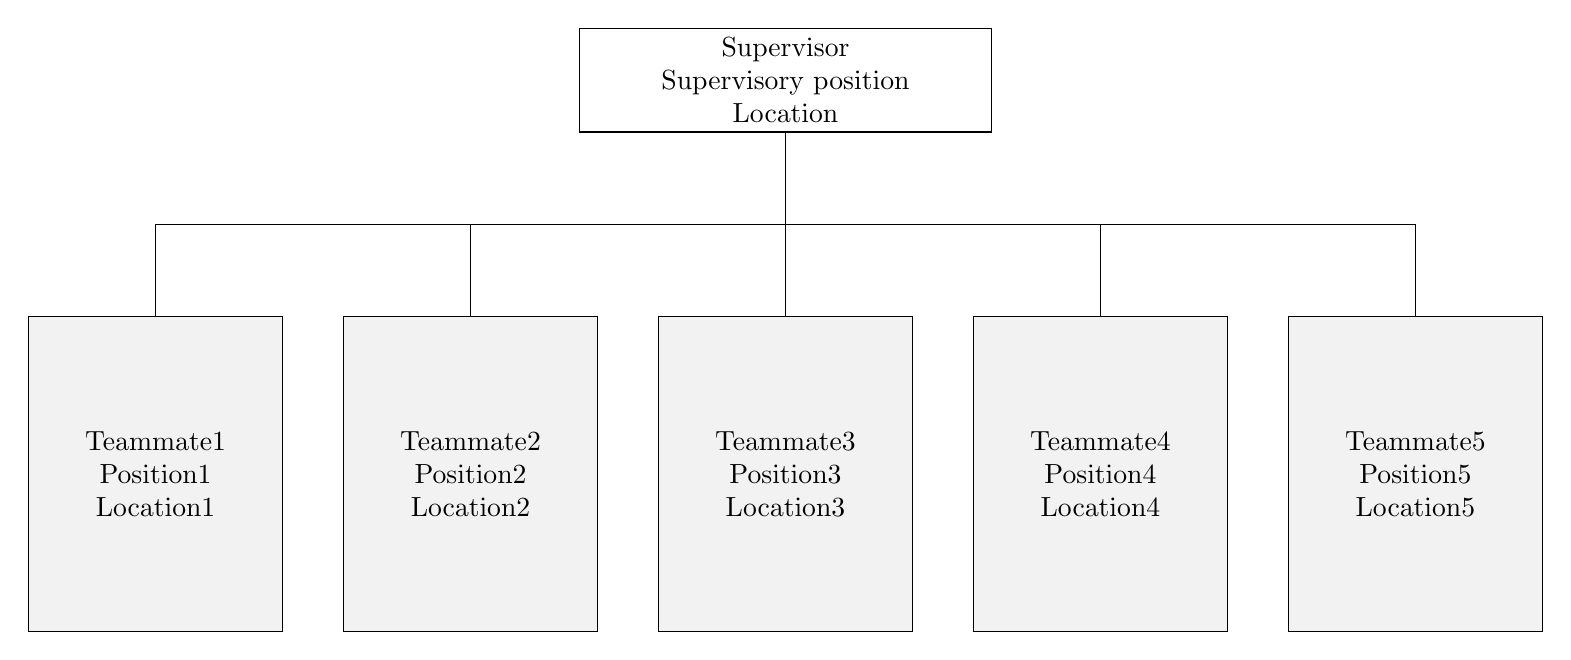
\begin{tikzpicture}[
    nodes={draw=black, thin,minimum height=3em},
    supervisor/.style={%
        text centered, text width=5cm},
    teammate/.style={%
        text centered, text width=3cm,
        minimum height=4cm,
        fill=gray!10},
    level 1/.style={sibling distance=4cm,level distance=5cm},
]
     %Supervisor
    \node[anchor=south,supervisor]{Supervisor\\Supervisory position\\Location}
    [my edge from parent fork down]
     %Teammate
    child{node [teammate] {Teammate1\\Position1\\Location1}}
    child{node [teammate
        %,minimum height=2cm
    ] {Teammate2\\Position2\\Location2}}
    child{node [teammate] {Teammate3\\Position3\\Location3}}
    child{node [teammate] {Teammate4\\Position4\\Location4}}
    child{node [teammate] {Teammate5\\Position5\\Location5}}
;
\end{tikzpicture}
\end{document}